% This LaTeX document needs to be compiled with XeLaTeX.
%\documentclass[10pt]{article}
%\usepackage[utf8]{inputenc}
%\usepackage{ucharclasses}
%\usepackage{amsmath}
%\usepackage{amsfonts}
%\usepackage{amssymb}
%\usepackage[version=4]{mhchem}
%\usepackage{stmaryrd}
%\usepackage{graphicx}
%\usepackage[export]{adjustbox}
%\graphicspath{ {./images/} }
%\usepackage{polyglossia}
%\usepackage{fontspec}
%\setmainlanguage{hindi}
%\setotherlanguages{english}
%\IfFontExistsTF{Noto Serif Devanagari}
%{\newfontfamily\hindifont{Noto Serif Devanagari}}
%{\IfFontExistsTF{Kohinoor Devanagari}
%  {\newfontfamily\hindifont{Kohinoor Devanagari}}
%  {\IfFontExistsTF{Devanagari MT}
%    {\newfontfamily\hindifont{Devanagari MT}}
%    {\IfFontExistsTF{Lohit Devanagari}
%      {\newfontfamily\hindifont{Lohit Devanagari}}
%      {\IfFontExistsTF{FreeSerif}
%        {\newfontfamily\hindifont{FreeSerif}}
%        {\newfontfamily\hindifont{Arial Unicode MS}}
%}}}}
%\IfFontExistsTF{CMU Serif}
%{\newfontfamily\lgcfont{CMU Serif}}
%{\IfFontExistsTF{DejaVu Sans}
%  {\newfontfamily\lgcfont{DejaVu Sans}}
%  {\newfontfamily\lgcfont{Georgia}}
%}
%\setDefaultTransitions{\lgcfont}{}
%\setTransitionsForDevanagari{\hindifont}{\rmfamily}

\documentclass[10pt]{article}
\usepackage[utf8]{inputenc}
\usepackage[T2A]{fontenc} % если нужна кириллица
\usepackage[russian,english]{babel} % если нужна кириллица
\usepackage{amsmath}
\usepackage{amsfonts}
\usepackage{amssymb}
\usepackage[version=4]{mhchem}
\usepackage{stmaryrd}
\usepackage{graphicx}
\usepackage[export]{adjustbox}
\graphicspath{{./images/}}

\begin{document}
\begin{itemize}
  \item havckas \(e^{i \vec{k} \cdot \vec{x}}\)
  \item сорериr \(\frac{e^{i k \cdot r}}{r}\)\\
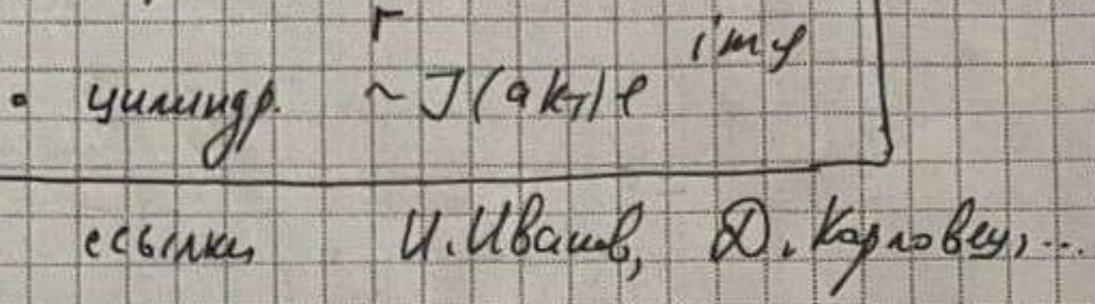
\includegraphics[max width=\textwidth, center]{2025_07_22_dcbd22cba3b771cfb453g-01(3)}\\
\(\rightarrow\) мриотовито Jangy. cocm.\\
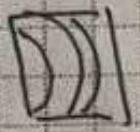
\includegraphics[max width=\textwidth, center]{2025_07_22_dcbd22cba3b771cfb453g-01(1)}\\
\(\rightarrow\) pacnag Xunca\\
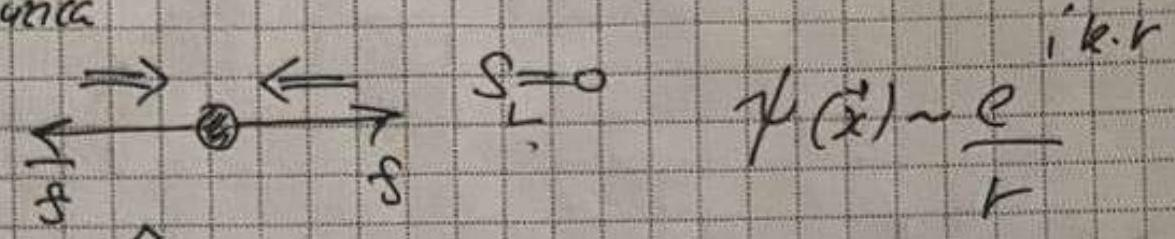
\includegraphics[max width=\textwidth, center]{2025_07_22_dcbd22cba3b771cfb453g-01(2)}
\end{itemize}

\[
\overbrace{\forall}^{z \uparrow} \int_{f=+1, L_{z}=-1}^{\prod_{L}} S_{T}=1
\]

\begin{center}
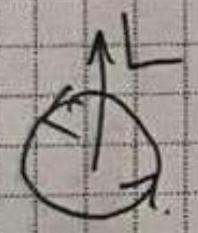
\includegraphics[max width=\textwidth]{2025_07_22_dcbd22cba3b771cfb453g-01}
\end{center}

\[
\begin{aligned}
& \psi\left(\vec{r}_{1}, \vec{r}_{2}\right)=\int \frac{d^{3} p_{1} d_{2} p_{2} \psi\left(\vec{h}_{1} \vec{p}_{2}\right)}{\left.(2 \pi)^{6} \sqrt{2 E_{p} r_{1}}\right) e^{i(i)}} \\
& =\int d^{2} p d^{2} p t\langle f f \mid S-1\rangle e^{i(1)}
\end{aligned}
\]

\[
\begin{aligned}
& \left.-\delta^{3}\left(\vec{p}_{1}-\vec{p}_{2}\right) \delta^{\prime}\left(\vec{p}_{2}-\vec{p}_{1}^{\prime}\right)\right]
\end{aligned}
\]

\[
\begin{aligned}
& |\vec{p}\rangle \equiv \sqrt{2 E_{p}} a_{p}^{+}(0\rangle \\
& \langle\vec{q} \mid \vec{p}\rangle=\langle\vec{q}| a_{q} \sqrt{2 E_{q}} \sqrt{2 F_{p}} a_{p}^{+}(0)=2 E_{p}(2 \pi)^{3} \delta^{3}(\vec{q} \cdot \vec{p}) \\
& a_{q} a_{p}^{+}=a_{p}^{+} a_{q}+\left[a_{t}, a_{p}^{+}\right] \\
& \text {(2Ti) } \operatorname{Los}^{3} \delta^{3}(\vec{q}-\vec{p}) \\
& \langle\vec{q}, s \mid \vec{p}, r\rangle=2 E_{p}(2 \pi)^{3} \delta^{s}(\vec{q} p) \delta_{s r} \\
& \left|\vec{p}_{1, p p_{2}}\right\rangle=\sqrt{2 E_{1} 2 E_{p 2}} a_{p 1 s_{1}}^{+} a_{p p_{2} s_{2}}^{+}|0\rangle \\
& \left\langle q_{1}, r_{1} ; q_{2}, r_{2} \mid p s_{1} ; p_{2} s_{2}\right\rangle=\sqrt{2 E_{p}, 2 E_{p} 2 E_{q}, 2 E_{q 2}} \times \\
& \begin{aligned}
x<0 \mid a_{q_{1} r_{1}} & \frac{a_{q_{2} r_{2}}}{a_{p r_{1} r_{1}}} a_{q r_{2}}^{+}+\left[a_{q r_{2}}, a_{p r_{2}}^{+}|0\rangle\right.
\end{aligned} \\
& z\langle 0| a_{q_{1} r_{1}}\left(a_{p 1_{1} 1_{1}}^{+} a_{q_{2} 1_{2}}+\left[a_{q_{2} r_{2}}, a_{p, 5}^{+}\right]\right) a_{p \delta_{2}}^{+}|0\rangle \\
& =\left[a_{q_{2 \mid 2}}, a_{p, s_{1}}^{+}\right]<\underbrace{\left\langle 0 \mid a_{q \mid r_{1}} a_{p, r_{2} \mid 0}^{+}\right\rangle}_{\left[a_{q, r_{1}}, a_{p, s_{2}}^{+}\right]} \\
& \begin{array}{l}
+\langle 0| a_{q_{1} r_{1}} a_{p r_{1}}^{+}\left(a_{p r_{2}}^{+} a_{q_{2} r_{2}}+\left[a_{q r_{2}}, a_{p r_{2}}^{+}\right]|0\rangle\right. \\
=\left[a_{q r_{2}}, a_{p r_{1}}^{+}\right]\left[a_{q r_{1}}, a_{p r_{2}}^{+}\right]+\left[a_{q r_{2}}, a_{p r_{2}}^{+}\right]\left[a_{q r_{1}}, a_{p p_{2}}^{+}\right]
\end{array} \\
& \left\langle\vec{q}_{1} r_{1} ; \vec{q}_{2} r_{2}\right| s|H\rangle=\int \frac{d^{3} p_{1} d^{3} p_{2}}{(2 \pi)^{6}} \sqrt{2 E_{p} r_{2}^{2} p_{2}} \tilde{\psi}\left(\vec{p}_{1} \vec{p}_{2}\right)\left\langle q_{1} r_{1} q_{2} r_{2}\right| p_{1} p_{1}^{2}\left|p_{1}\right| \\
& \begin{array}{r}
=\int \frac{d^{3} r_{2} d^{3} p_{2}}{(2 \pi)^{6} \Sigma_{2} F_{2} F_{2}} \tilde{\psi}\left(\bar{p}_{1} \bar{p}_{2}\right)\left[(2 \pi)^{6} \delta^{3}\left(q_{2}-p_{1}\right) \delta_{r_{2} s}, \delta^{3}\left(q_{1}-p_{2}\right) \delta_{r_{1} s_{2}}\right. \\
\left.+(2 \pi)^{6} q_{2} \delta^{3}\left(q_{2}-p_{2}\right) \delta_{r_{2} \delta_{2}} \delta^{3}\left(\phi_{1}-p_{2}\right) \delta_{r_{1} s}\right]
\end{array} \\
& =\frac{\tilde{\Psi}\left(q_{2}, q_{1}\right)}{\sqrt{2 E_{1} 2 E_{92}}} \delta_{r_{2} s_{1} \delta r_{1} s_{2}}+\frac{\tilde{\psi}\left(q_{1}, q_{1}\right)}{\sqrt{2 E_{1}, 2 E_{12}}} \delta_{n s_{1} \delta r_{2} \delta v}
\end{aligned}
\]

\[
\begin{aligned}
& |\vec{p}\rangle \equiv \sqrt{2 E_{p}} a_{p}^{+}(0\rangle \\
& \langle\vec{q} \mid \vec{p}\rangle=\langle\vec{q}| a_{q} \sqrt{2 E_{q}} \sqrt{2 F_{p}} a_{p}^{+}(0)=2 E_{p}(2 \pi)^{3} \delta^{3}(\vec{q} \cdot \vec{p}) \\
& a_{q} a_{p}^{+}=a_{p}^{+} a_{q}+\left[a_{t}, a_{p}^{+}\right] \\
& \text {(2Ti) } \operatorname{Los}^{3} \delta^{3}(\vec{q}-\vec{p}) \\
& \langle\vec{q}, s \mid \vec{p}, r\rangle=2 E_{p}(2 \pi)^{3} \delta^{s}(\vec{q} p) \delta_{s r} \\
& \left|\vec{p}_{1, p p_{2}}\right\rangle=\sqrt{2 E_{1} 2 E_{p 2}} a_{p 1 s_{1}}^{+} a_{p p_{2} s_{2}}^{+}|0\rangle \\
& \left\langle q_{1}, r_{1} ; q_{2}, r_{2} \mid p s_{1} ; p_{2} s_{2}\right\rangle=\sqrt{2 E_{p}, 2 E_{p} 2 E_{q}, 2 E_{q 2}} \times \\
& \begin{aligned}
x<0 \mid a_{q_{1} r_{1}} & \frac{a_{q_{2} r_{2}}}{a_{p r_{1} r_{1}}} a_{q r_{2}}^{+}+\left[a_{q r_{2}}, a_{p r_{2}}^{+}|0\rangle\right.
\end{aligned} \\
& z\langle 0| a_{q_{1} r_{1}}\left(a_{p 1_{1} 1_{1}}^{+} a_{q_{2} 1_{2}}+\left[a_{q_{2} r_{2}}, a_{p, 5}^{+}\right]\right) a_{p \delta_{2}}^{+}|0\rangle \\
& =\left[a_{q_{2 \mid 2}}, a_{p, s_{1}}^{+}\right]<\underbrace{\left\langle 0 \mid a_{q \mid r_{1}} a_{p, r_{2} \mid 0}^{+}\right\rangle}_{\left[a_{q, r_{1}}, a_{p, s_{2}}^{+}\right]} \\
& \begin{array}{l}
+\langle 0| a_{q_{1} r_{1}} a_{p r_{1}}^{+}\left(a_{p r_{2}}^{+} a_{q_{2} r_{2}}+\left[a_{q r_{2}}, a_{p r_{2}}^{+}\right]|0\rangle\right. \\
=\left[a_{q r_{2}}, a_{p r_{1}}^{+}\right]\left[a_{q r_{1}}, a_{p r_{2}}^{+}\right]+\left[a_{q r_{2}}, a_{p r_{2}}^{+}\right]\left[a_{q r_{1}}, a_{p p_{2}}^{+}\right]
\end{array} \\
& \left\langle\vec{q}_{1} r_{1} ; \vec{q}_{2} r_{2}\right| s|H\rangle=\int \frac{d^{3} p_{1} d^{3} p_{2}}{(2 \pi)^{6}} \sqrt{2 E_{p} r_{2}^{2} p_{2}} \tilde{\psi}\left(\vec{p}_{1} \vec{p}_{2}\right)\left\langle q_{1} r_{1} q_{2} r_{2}\right| p_{1} p_{1}^{2}\left|p_{1}\right| \\
& \begin{array}{r}
=\int \frac{d^{3} r_{2} d^{3} p_{2}}{(2 \pi)^{6} \Sigma_{2} F_{2} F_{2}} \tilde{\psi}\left(\bar{p}_{1} \bar{p}_{2}\right)\left[(2 \pi)^{6} \delta^{3}\left(q_{2}-p_{1}\right) \delta_{r_{2} s}, \delta^{3}\left(q_{1}-p_{2}\right) \delta_{r_{1} s_{2}}\right. \\
\left.+(2 \pi)^{6} q_{2} \delta^{3}\left(q_{2}-p_{2}\right) \delta_{r_{2} \delta_{2}} \delta^{3}\left(\phi_{1}-p_{2}\right) \delta_{r_{1} s}\right]
\end{array} \\
& =\frac{\tilde{\Psi}\left(q_{2}, q_{1}\right)}{\sqrt{2 E_{1} 2 E_{92}}} \delta_{r_{2} s_{1} \delta r_{1} s_{2}}+\frac{\tilde{\psi}\left(q_{1}, q_{1}\right)}{\sqrt{2 E_{1}, 2 E_{12}}} \delta_{n s_{1} \delta r_{2} \delta v}
\end{aligned}
\]

\[
\begin{aligned}
& \left\langle 0 a_{a} a_{p,}^{+} a_{p}^{+} \mid 0\right\rangle=[,]\langle\underbrace{0 \mid a^{+}}_{\varnothing}| \nu+\langle 0| a^{+} \underbrace{0}_{a^{+} a+5,} a^{+}|0\rangle \\
& a^{+} a+[1] \\
& =\frac{\tilde{\psi}\left(q_{2} r_{2} ; q_{1} r_{1}\right)+\tilde{\psi}\left(q_{1} r_{1} ; q_{2} r_{2}\right)}{\sqrt{2 \varepsilon_{1} 2 E_{\varepsilon_{2}}}} \\
& \left\{a_{p s}, a_{q r}^{+}\right\}=(2 \pi)^{3} \delta^{3}(p-q) \delta_{s v} \\
& a_{p s} a_{q r}^{t} \varepsilon=-a_{q r}^{t} a_{p s}+\{,\} \\
& \widetilde{\psi}\left(q_{1} r_{1} ; q_{2} r_{2}\right) \sim \sqrt{2 E_{1} 2 E_{1}}\left\langle q_{1} r_{1} ; q_{2} r_{2}\right| S-1|H\rangle \\
& \psi\left(\vec{r}_{1}, s_{1} ; \vec{r}_{2} ; \dot{s}_{2}\right)=\int \frac{d^{3} p_{1} d^{2} h\left(\widetilde{\psi}\left(p_{1} s_{1} ; p_{2} r_{2}\right) e^{i}(2 \pi)^{2} \sqrt{2 E_{p}, 2 E_{p}}\right.}{(2 \pi)} \\
& x e^{+i \vec{p}_{1}, \vec{r}_{1}+i \vec{p}_{2} \cdot \vec{r}_{2}} \\
& =\int \frac{d^{3} p_{1} d^{3} n}{(2 \pi)^{6}} \underbrace{\left\langle q p_{1} s_{1} ; p_{2} s_{1}\right| S-1|H\rangle} e \\
& \left.(2 \pi)^{4} \delta^{4}\left(P_{H}-P_{1}-P_{2}\right) ; \frac{M_{3}}{v} \bar{u}\left(P_{1} S_{1}\right)\right\}\left(p_{2} s_{2}\right) \\
& u(\vec{p}, \vec{s})=\left(\begin{array}{ll}
\sqrt{E_{p}+m} \chi(\vec{p}, \vec{s}) & \vec{r} \cdots H \\
\sqrt{E_{p}-m} \vec{\sigma}, \hat{n}_{p} \chi(\vec{r}, \vec{s})
\end{array}\right) \quad \\
& \bar{u}=u^{\dagger} \gamma_{0}=\left(\sqrt{E_{p}+m} \chi^{+}(p, s), \sqrt{E_{p}-m} \tilde{\xi}_{0} \cdot \int^{+}(p, s) \tilde{\sigma}^{-} \hat{n}_{p}\right) \\
& x\left(\begin{array}{cc}
1 & 0 \\
0 & -1
\end{array}\right)=\left(\sqrt{E_{p}+m} X^{t},-\sqrt{E_{1}-m} X^{t} \sigma \cdot n\right)
\end{aligned}
\]

\[
\begin{aligned}
& =\left.\int \frac{d^{2} p_{1}}{(2 \pi)^{6}} \delta\left(m_{H}-E_{p_{1}}-E_{1 i}\right) i \frac{m_{1}}{z} \bar{u}\left(p_{1} s_{1}\right) z\left(p_{2} s_{2}\right)\right|_{\vec{p}_{2}=-\vec{p}_{1}} ^{(\cdots \cdots)} \\
& d^{3} P_{1}=\underbrace{P_{1}^{2} d P_{1}} d P_{1} \\
& P_{1} E_{1} d E_{1} \\
& l_{1} d_{p}=p_{1} p_{1} d_{p}=p_{1} E_{1} d E_{1} \\
& \left.E^{2}=P^{2}+m^{2}, E d E=P d P\right\}=\sqrt{E^{2}-m^{2}} E_{1} d E_{1} \\
& =\frac{1}{(2 \pi)^{6}} \int d \Omega p_{1} \sqrt{E_{1}^{2}-m^{2}} E_{1} \delta\left(m_{H}-2 E_{1}\right) i \frac{m_{+}}{v} \bar{u}\left(p_{1} s_{1}\right) v\left(-1, p_{2}\right) \\
& \begin{array}{r}
\left.=\frac{1}{(2 \pi)^{6}} \frac{1}{2} \int \phi \Omega_{1} \sqrt{\left(\frac{M H}{2}\right)^{2}-m^{2}} \frac{m_{H}}{2}: \left.\frac{M+}{v} \vec{u}\left(\vec{P}_{1} s_{1}\right) z \right\rvert\,-\vec{P}_{1} s_{2}\right)\left.\right|_{\left|\vec{P}_{1}\right|=} \\
=\sqrt{\left(\frac{N}{2}\right)^{2} \cdot u^{1}}
\end{array} \\
& \int d x f(x) g\left(x \delta(g(x))=\sum_{i} \frac{f\left(x_{i}\right)}{\left|g^{\prime}\left(x_{i}\right)\right|}\right. \\
& \begin{array}{l}
g \equiv M_{H}-R E_{1} \equiv g\left(E_{1}\right), g^{\prime}\left(E_{1}\right)=-2 \\
\geqslant X(\vec{n}, \vec{s})=\left(\cos \frac{t}{2}, \mu^{\wedge}=\frac{\vec{p}}{|\vec{p}|}\right.
\end{array} \\
& 11\left(+\sin \frac{\theta}{2} e^{1 \varphi}\right) \\
& \psi\left(\bar{r}_{1}-\bar{r}_{2}, s_{1} s_{2}\right) \sim \int d \theta \sin \theta d \varphi \quad \underbrace{\prime \prime}(\theta, \varphi) e^{i \vec{p} \mid\left(\vec{r}_{1}-\vec{r}_{2}\right) \cdot \hat{h}} \\
& \text { uv } e^{i(p) \overline{4} \hat{n}}
\end{aligned}
\]

\[
\begin{aligned}
& \left\langle\bar{p}_{1}^{\prime}, \bar{p}_{2}^{\prime} \mid \bar{p}_{1}, \bar{p}_{2}\right\rangle \\
& |p\rangle=\sqrt{2 E_{p}} a_{p}^{+}|0\rangle \\
& \langle\bar{q} \mid \bar{p}\rangle=\langle\bar{q}| a_{q} \sqrt{E_{q}} \sqrt{2 E_{p}} a_{p}^{+}|0\rangle \\
& \left\{a_{q}, a_{p}{ }^{+}\right\}=a_{q} a_{p}{ }^{+}+a_{q}{ }^{+} a_{p} \Rightarrow a_{q} a_{p}{ }^{+}=a_{q}{ }^{+} a_{p}+\left\{a_{q}, a_{p}{ }^{+}\right\} \\
& \langle\bar{q}, s \mid \bar{p}, r\rangle=2 E_{p}(2 \pi)^{3} \delta^{3}(\bar{q}-\bar{p}) d_{s r} \\
& \left\langle q_{1}, r_{1} ; q_{2}, r_{2} \mid p_{1} s_{1} j p_{2} s_{2}\right\rangle= \\
& =\sqrt{2 E_{p, 2} 2 E_{p 2} 2 E_{q, 2} 2 E_{q 2}} \times\langle 0| \quad a_{q, 4,} \underbrace{a_{q 2,4}} a_{p, 1,1}^{+} a_{p, 3,2}^{+}|0\rangle \\
& =\sqrt{2 E_{p, 2} 2 E_{p 2} 2 E_{q, 2} 2 E_{q 2}}<01 a_{q 4_{1}}\left(-a_{q 4_{1}}^{+} a_{p 4_{1}}^{+}\left\{a_{q 4_{2}}, a_{p 5_{1}}^{+}\right\}\right) a_{p 5_{2}}^{+}(0)=
\end{aligned}
\]

\[
\begin{aligned}
& \text { ? } \\
& =\left\{a_{q, v} a_{p, s}^{+} s-\left\{a_{q, r_{1}, a_{p, s}}^{+}\right\}-\left\{a_{q, r_{1}} a_{q, r_{2}}^{+}\right\}\left\{a_{p, s, a_{p, s}}\right\}\right. \\
& \left\langle\bar{q}_{1} u_{1} ; \bar{q}_{2} u_{2}\right| S|H\rangle=\int \frac{d^{3} p_{1} d^{3} p_{2}}{(2 \pi)^{6} \sqrt{2 E_{p, 2} \epsilon_{p}}} \tilde{\Psi}\left(\overline{p_{1}}, \overline{p_{2}}\right) x \\
& x\left\langle q_{1} r_{1} ; q_{2} r_{2} \mid p_{1} s_{1} ; p_{2} s_{2}\right\rangle= \\
& =\int \frac{d^{3} p_{1} d^{3} p_{2}}{(2 \pi)^{2} \sqrt{2 E, 2 E 2}} \bar{\psi}\left(\bar{p}_{1} \bar{p}_{2}\right) L(2 \pi)^{6} \delta^{(3)}\left(q_{2}-p_{1}\right) \partial_{r 2 s_{1} x} \\
& \times d^{3}\left(q_{1}-p_{1}\right) d_{4, s_{2}}= \\
& \text { - (20) }{ }^{r}{ }^{(3)}\left(q_{2}-p_{2}\right) \partial_{223} x \\
& x \delta^{3}\left(q_{1}-p_{1}\right) \delta_{r, s .}
\end{aligned}
\]

\[
\begin{aligned}
\bar{u}= & \left(\sqrt{E_{p}+m} x^{+},-\sqrt{E_{p}-m} x^{+} \sigma \cdot n\right)= \\
= & \left(\sqrt{E_{p}+m}\left(\cos \frac{\theta}{2}, e^{i p} \sin \frac{\theta}{2}\right),\right. \\
& \left.-\sqrt{E_{p}-m}\left(\cos \frac{\theta}{2}, e^{i \varphi} \sin \frac{\theta}{2}\right) \bar{\sigma}-\hat{n}\right)
\end{aligned}
\]

\[
v=\binom{\sqrt{E_{p}+m} \quad x(-\bar{B}, \bar{s}),}{\sqrt{E_{p}-m} \bar{\sigma} \cdot \hat{n}_{p} x\left(-\bar{p}_{2}, \bar{s}_{2}\right)}=
\]

\begin{enumerate}
  \setcounter{enumi}{32}
  \item \(\left.\quad \sqrt{\bar{E}_{p}-m} \bar{\sigma} \cdot \hat{n}_{p}\left(\sin ^{2} \bar{c}_{p}\right)^{2}\right) \quad \underline{n}_{p}=(\sin \theta \cos p\), \(\sin \theta \sin p_{1}\) \(\cos \theta)\)
\end{enumerate}

\[
\begin{aligned}
\bar{\omega} \sigma= & \left(\sqrt{E_{p}+m} \cos \frac{\theta}{2}, \sqrt{E_{p}+m} e^{i \varphi} \sin \frac{\theta}{2}\right. \\
& \left.-\sqrt{E_{p}-m} \cos \frac{\theta}{2} \overline{\sigma \cdot \hat{n}},-\sqrt{E_{p}-m} e^{i p} \sin \frac{\theta}{2} \frac{\theta}{\sigma \cdot \hat{n}}\right) . \\
\times & \left(\begin{array}{l}
\sqrt{E_{p}+m} \cos \frac{\theta}{2} \\
\sqrt{E_{p}+m} \sin \frac{\theta}{2} e^{i p} \\
\sqrt{E_{p}-m} \frac{\theta}{\epsilon} \cdot \hat{n}_{p} \cos \frac{\theta}{2} \\
\sqrt{E_{p}-m} \bar{\sigma} \cdot \hat{n}_{p} \sin \frac{\theta}{2} e^{i p}
\end{array}\right) \\
\bar{u} \bar{\theta}- & \left(\sigma_{p}+m\right) \cos ^{2} \frac{\theta}{2}+\left(E_{p}+m\right) \\
\bar{u} \theta= & \left(E_{p}+m\right) \cos ^{2} \frac{\theta}{2}+\left(E_{p}+m\right) e^{2 i \varphi} \sin ^{2} \frac{\theta}{2}- \\
& -\left(E_{p}-m\right)(\hat{\sigma} \cdot \hat{n})^{2} \cos ^{2} \frac{\theta}{2}-\left(E_{p}-m\right) e^{2 i p} \sin \frac{\theta}{2}\left(\hat{\sigma} \cdot \hat{n}_{p}\right)^{2}
\end{aligned}
\]

\[
\begin{aligned}
& x^{+}\left(\bar{s}_{1}\right) \hat{n} \cdot \bar{\sigma} q\left(\bar{s}_{2}\right) \\
& \bar{n}=\left(\sin \theta \cos \varphi_{0} \sin \theta \sin \varphi_{0} \cos \theta\right) \\
& \hat{s}_{i}=\left(\sin \theta_{i} \cos p_{i}, \sin \theta_{i} \sin p_{i} \cos \theta_{i}\right) \\
& \bar{r}=r\left(\sin \theta_{r} \cos p_{r}, \sin \theta_{r}\right. \text {. } \\
& \hat{n} \cdot \bar{\sigma}=n_{1} \sigma_{1}+n_{2} \sigma_{2}+n_{3} \sigma_{3}= \\
& =\left(\begin{array}{cc}
0 & \sin \theta \cos \phi \\
\sin \theta \cos \phi & 0
\end{array}\right)+\left(\begin{array}{cc}
0 & -i \sin \theta \sin \phi \\
i \sin \theta \sin p & 0
\end{array}\right)+\left(\begin{array}{cc}
\cos \theta & 0 \\
0 & -\cos \theta
\end{array}\right)= \\
& =\left(\begin{array}{cc}
\cos \theta & \sin \theta e^{-i \varphi} \\
\sin \theta e^{-i \varphi}-\cos \theta
\end{array}\right) \\
& \eta\left(\vec{s}_{2}\right)=\cos \frac{\theta_{3}}{2}\binom{1}{0}+\sin \frac{\theta_{2}}{2} e^{i \phi_{2}}\binom{0}{1}=\binom{\cos \frac{\theta_{3}}{2}}{\sin \frac{\theta_{1}}{2} e^{i p_{2}}} \\
& \bar{n} \cdot \bar{\sigma} \eta\left(s_{2}\right)=\left(\begin{array}{cc}
\cos \theta & \sin \theta e^{-i \varphi} \\
\sin \theta e^{i \varphi} & -\cos \theta
\end{array}\right)\binom{\cos \frac{\theta_{2}}{2}}{\sin \frac{\theta_{2}}{2} e^{i \phi_{2}}}= \\
& =\cos \theta \cos \frac{\theta_{2}}{2}+\sin \theta \sin \frac{\theta_{2}}{2} / e^{i\left(p_{2}-p\right)}+ \\
& +\sin \theta \varphi^{2} \sin \theta e^{i \varphi} \cos \frac{\theta_{2}}{2}-\cos \theta \sin \frac{\theta_{2}}{2} e^{i \varphi_{2}} \\
& =\cos \frac{\theta_{2}}{2}\binom{\cos \theta}{\sin \theta c^{i \varphi}}+\sin ^{\frac{\theta_{2}}{2}} e^{i \varphi_{2}}\binom{\sin \theta e^{-\dot{\varphi}}}{-\cos \theta} \\
& \lambda^{+}\left(\bar{s}_{1}\right) \bar{n} \bar{\sigma} \cdot \eta\left(\bar{s}_{2}\right)=\left[\cos \frac{\partial_{1}}{2}\binom{1}{0}+\sin \frac{\partial_{1}}{2} e^{\left.-i \varphi \cdot\binom{0}{1}\right] x}\right. \\
& x\left[\cos \frac{\theta_{2}}{2}\left(\cos \theta i \sin \theta e^{i \varphi}\right)+\sin \frac{\theta_{1}}{2} e^{i \varphi}\left(-\sin \theta e^{-i}{ }^{\top}-\cos \theta\right)\right]
\end{aligned}
\]

\(=\cos \frac{\theta_{1}}{2} \cos \frac{\theta_{2}}{2} \cos \theta_{p}+\cos \frac{\theta_{1}}{2} \sin \frac{\theta_{2}}{2} e^{i p_{2}} \sin \theta_{p} e^{i-i p_{+}}\) \(\sin \frac{\partial_{1}}{2} \cos \frac{\partial_{2}}{2} \sin \theta_{p} c^{\varphi_{p}}-\sin \frac{\theta_{1}}{2} \sin \frac{\theta_{2}}{2} e^{i\left(\varphi_{1}+\varphi_{1}\right)_{c}^{p}}\) \(+\sin \frac{\partial_{1}}{2} \cos \frac{\partial_{2}}{2} \sin \theta_{p} e^{u p_{p}} e^{-\bar{i}_{p_{1}}} \sin \frac{\theta_{1}}{2} \sin \frac{\theta_{2}}{2} e^{i\left(\varphi_{1} p_{1}\right)} \cos \theta_{p}\)

\[
\begin{aligned}
& e^{i \bar{p} \cdot \bar{r}}=\sum_{e=0}^{\infty} i^{e} j e(p r) P e(\cos \theta)(2 l+1) \\
& \int d \hat{n} x^{+}\left(\overline{s_{1}}\right) \hat{n} \bar{\sigma} \eta\left(\overline{s_{2}}\right) e^{i \bar{p} \cdot \bar{r}}= \\
& =2 \pi \int_{-1}^{1} d \cos \theta[\cos \theta] \sum_{c=0}^{\infty} i^{e} j e(p r) P e(\cos \theta) x \\
& \quad x\left[\cos \frac{\theta_{1}}{2} \cos \frac{\theta_{2}}{2}-\sin \frac{\theta_{1}}{2} \sin \frac{\theta_{2}}{2} e^{i\left(p_{2}-p_{1}\right)}\right]
\end{aligned}
\]

\[
\int_{-1}^{\text {OpTonoualbuoct }} P_{m}(x) P_{n}(x) d x=\frac{2}{n+1} \int_{m n} \quad \int_{-1}^{1} P_{k}(x) d x=\left\{\begin{array}{l}
2, k=0 \\
0, k \geq 1
\end{array}\right.
\]

%\(u_{3}\) - उद орто zoulloudici преоразубета

\[
\begin{gathered}
x P_{c}(x)=\frac{e_{1}}{2 e+1} P_{e+1}(x)+\frac{e}{2 c+1} P_{e-1}(x) \\
\int_{-1}^{1} x P_{e}(x) d x=\int_{-1}^{1}\left(\frac{e}{2 c+1} P_{e-1}(x)+\frac{c+1}{2 c+1} P_{c+1}(x)\right) d x
\end{gathered}
\]

He paba uyive npu \(e=1\)

\[
\begin{aligned}
\int_{-1}^{1} d p_{1}(x) d x & =\int_{-1}^{1}\left(\frac{4}{3} p_{0}(x)+\frac{2}{3} p_{2}(x)\right) d x= \\
& =\frac{1}{3} \cdot 2+\frac{2}{3} \cdot 0=\frac{2}{3} \\
\int_{-1}^{1} d \cos \theta \cos \theta & p_{e}(\cos \theta)=\frac{2}{3} \gamma_{e 1}
\end{aligned}
\]

\[
\begin{aligned}
& \Leftrightarrow 2 \pi\left[\cos \frac{\theta_{1}}{2} \cos \frac{\theta_{2}}{2}-\sin \frac{\theta_{1}}{2} \sin \frac{\theta_{2}}{2} e^{i\left(p_{1}-p_{1}\right)}\right] \sum_{e=0}^{\infty} i^{2} j\left(p_{1}\right) x \\
& -x \int_{-1}^{1} \cos \theta_{p} P_{c}(\cos \theta) d \cos \theta= \\
& =2 \pi[\ldots] \sum_{e=0}^{\infty} i_{j e}(p r) \cdot \frac{2}{3} \varepsilon_{e 1}= \\
& =2 \pi[\ldots] i_{11}(p r)^{\frac{2}{3}}= \\
& =\frac{4 \pi i}{3} j=(p r)\left[\cos \frac{\theta_{1}}{2} \cos \frac{\theta_{2}}{2}-\sin \frac{\theta_{1}}{2} \sin \frac{\theta_{2}}{2} e^{i\left(p_{2}-p_{1}\right)}\right]= \\
& =\frac{4 \pi i}{3}\left(\frac{\sin (p 4)}{(p)^{2}}-\frac{\sin (p 4)}{3_{2}}\right)\left[\cos \frac{\theta_{1}}{2} \cos \frac{\theta_{2}}{2}-\right. \\
& \stackrel{3_{f}^{2}}{\longleftrightarrow} \stackrel{s_{1}}{\longleftrightarrow}{ }_{f} \\
& \left.-\sin \frac{\theta_{1}}{2} \sin \frac{\theta_{1}}{2} e^{i\left(\varphi_{2}-\varphi_{1}\right)}\right] \\
& \stackrel{\Lambda^{s_{2}}}{\underset{\|}{\|} \xrightarrow{s_{1}}} \\
& \text {  }
\end{aligned}
\]

\[
\int_{0}^{\pi} \int_{0}^{2 \pi} y_{l}^{m} y_{l^{\prime}}^{m^{\prime} x} d r=\frac{4 \pi}{(2 l+1)} d_{l^{\prime}} d_{\text {men }}
\]

\(\int_{0}^{2 \pi} d p_{p} \int_{0}^{\pi} d \theta_{p} \sin \theta_{p} e^{i \bar{p} \cdot \bar{e}} x\)\\
\(x\left[\cos \frac{\theta_{1}}{2} \cos \frac{\theta_{2}}{2} \cos \theta_{p}+\cos \frac{\theta_{1}}{2} \sin \frac{\theta_{2}}{2} e^{i \varphi_{2}} \sin \theta e^{-i \varphi_{p}}+\right.\)\\
\(\left.+\sin \frac{\theta_{1}}{2} \cos \frac{\theta_{2}}{2} \sin \theta_{p} e^{i \varphi_{p}} e^{-i \varphi_{1}}-\sin \frac{\theta_{1}}{2} \sin \frac{\theta_{2}}{2} e^{i\left(\varphi_{2}-p\right)} \cos \theta_{p}\right]\)\\
\(=\int d p_{p} \int d \theta_{p} \sum_{l=0}^{\infty} \sum_{m=-l}^{l} 4 \pi i^{l} j c(k r) y_{m}^{l}\left(\theta_{p} \phi_{p}\right) \ddot{y}_{m}^{l}\left(\theta_{u} \varphi_{u}\right)\)\\
\(\zeta y_{0}^{0}=\frac{1}{2} \sqrt{\frac{1}{x}} \quad y_{1}^{-1}\left(\neq \frac{1}{2} \sqrt{\frac{3}{2 x}} \sin \theta e^{-i \varphi}\right.\)\\
\(\bar{E} \cdot v=\left\{y_{1}^{0}=\frac{1}{2} \sqrt{\frac{3}{3}} \cos \theta y_{1}^{-1}=\frac{1}{2} \sqrt{\frac{3}{2 \pi}} \sin \theta e^{-\psi}\right\}\) \(y_{1}^{\prime}=\frac{-1}{2} \sqrt{\frac{3}{2 \pi}} \sin \theta e^{i \varphi}\)\\
\(=\int d p_{p} \int d \theta_{p} \sum_{l=0}^{\infty} \sum_{m=-l}^{l} \varphi \pi t_{l}^{l} l^{(k r)} y_{m}^{l}\left(\theta_{p}, p_{p}\right) y_{m}^{+l}\left(\theta_{u} p_{r}\right)\)\\
\(*\left[\cos \frac{\theta_{1}}{2} \cos \frac{\theta_{2}}{2} 2 \sqrt{\frac{\pi}{3}} y_{1}^{0}+\cos \frac{\theta_{1}}{2} \sin \frac{\theta_{2}}{2} 2 \sqrt{\frac{\pi}{3}} y_{1}^{-1}+\right.\) \(+(-2) \sqrt{\frac{2 \pi}{3}} \sin \frac{\theta_{1}}{2} \cos \frac{\theta_{2}}{2} e^{-i p_{1}} y_{1}^{\prime}-2 \sqrt{\frac{\pi}{3}} \sin \frac{\theta_{1}}{2} \sin \frac{\theta_{2}}{2} x\) \(\left.x e^{i\left(p_{2}-p_{0}\right)} y_{1}^{0}\right]\)\\
\(\int d p \int d \cos \theta p \quad y_{1}^{-1}=\frac{1}{2} \sqrt{\frac{3}{2 \pi}} \sin \theta e^{-i p}\)

\[
y_{0}^{0}=\frac{1}{2} \sqrt{\frac{1}{3}}
\]

\[
y_{1}^{-1}=2 \sqrt{21}, \cdots \theta C
\]

\(\int_{0}^{2 \pi} d \varphi_{p} \int_{0}^{\pi} d \theta_{p} \sin \theta_{p} \sum_{l=0}^{\infty} \sum_{m=-l}^{l} 4 \pi i^{l} j_{l}(k r) y_{l}^{m}\left(\theta_{p}, \varphi_{p}\right) y_{l}^{*} e^{m}\left(\theta_{r}, \varphi_{l}\right)\) \(e^{i \varphi_{2}}\)\\
\(x\left[\cos \frac{\theta_{1}}{2} \cos \frac{\theta_{2}}{2} 2 \sqrt{\frac{\pi}{3}} y_{1}^{\circ}+\cos \frac{\theta_{1}}{2} \sin \frac{\theta_{2}}{2} 2 \sqrt{\frac{\pi}{3}} y_{1}^{-1}+\right.\)\\
\(+(-2) \sqrt{\frac{2 \pi}{3}} \sin \frac{\theta_{1}}{2} \cos \frac{\theta_{2}}{2} e^{-i \varphi_{1}} y_{1}^{\prime}-\)\\
\(\left.-2 \sqrt{\frac{\pi}{3}} \sin \frac{\theta_{1}}{2} \sin \frac{\theta_{2}}{2} e^{i\left(\varphi_{2}-\varphi_{1}\right)} y_{1}^{0}\right]=\)\\
\(=\int_{0}^{2 \pi} d p_{p} \int_{0}^{\pi} d \theta_{p} \sin \theta_{p} \sum_{m=-1}^{1} 4 \pi i j_{1}(k r) Y_{1}^{m}\left(\theta_{p}, p_{p}\right) Y_{1}^{* m}\left(\theta_{1}, p\right)=\)

\begin{itemize}
  \item \([\cdots]=\)\\
\(\stackrel{4 \pi i j+\left(\omega_{2}\right)}{=} \int_{0}^{2 \pi} d p_{p} \int_{0}^{\pi} d \theta_{p} \sin \theta_{p} \mid y_{1}^{-1}\left(\theta_{p}, p_{p}\right) y_{1}^{*-1}\left(\theta_{1}, p_{1}\right) y_{1}^{-1} x\) \(x \cos \frac{\theta_{1}}{2} \sin \frac{\theta_{2}}{2} 2 \sqrt{\frac{\sqrt{\pi}}{3}}+\)
\end{itemize}

\[
\begin{aligned}
& +y_{1}^{0}\left(\theta_{p}, \varphi_{p}\right) y_{1}^{*}\left(\theta_{1}, \varphi_{2}\right) y_{1}^{0} x \\
& \times\left(\cos \frac{\theta_{1}}{2} \cos \frac{\theta_{2}}{2} 2 \sqrt{\frac{\pi}{3}}-2 \sqrt{\frac{\pi}{3}} \sin \frac{\theta_{1}}{2} \sin \frac{\theta_{2}}{2}\right. \\
& \left.e^{-i \varphi_{2}-\varphi_{1}}\right) \\
& +y_{1}^{*}\left(\theta_{p}, \varphi_{p}\right) y^{*} \frac{1}{1}\left(\theta_{1}, \varphi_{1}\right) y_{1}^{\prime} x \\
& \left.\times\left((-2) \sqrt{\frac{2 \pi}{3}} \sin \frac{\theta_{1}}{2} \cos \frac{\theta_{2}}{2} e^{-i \varphi_{1}}\right)\right]
\end{aligned}
\]

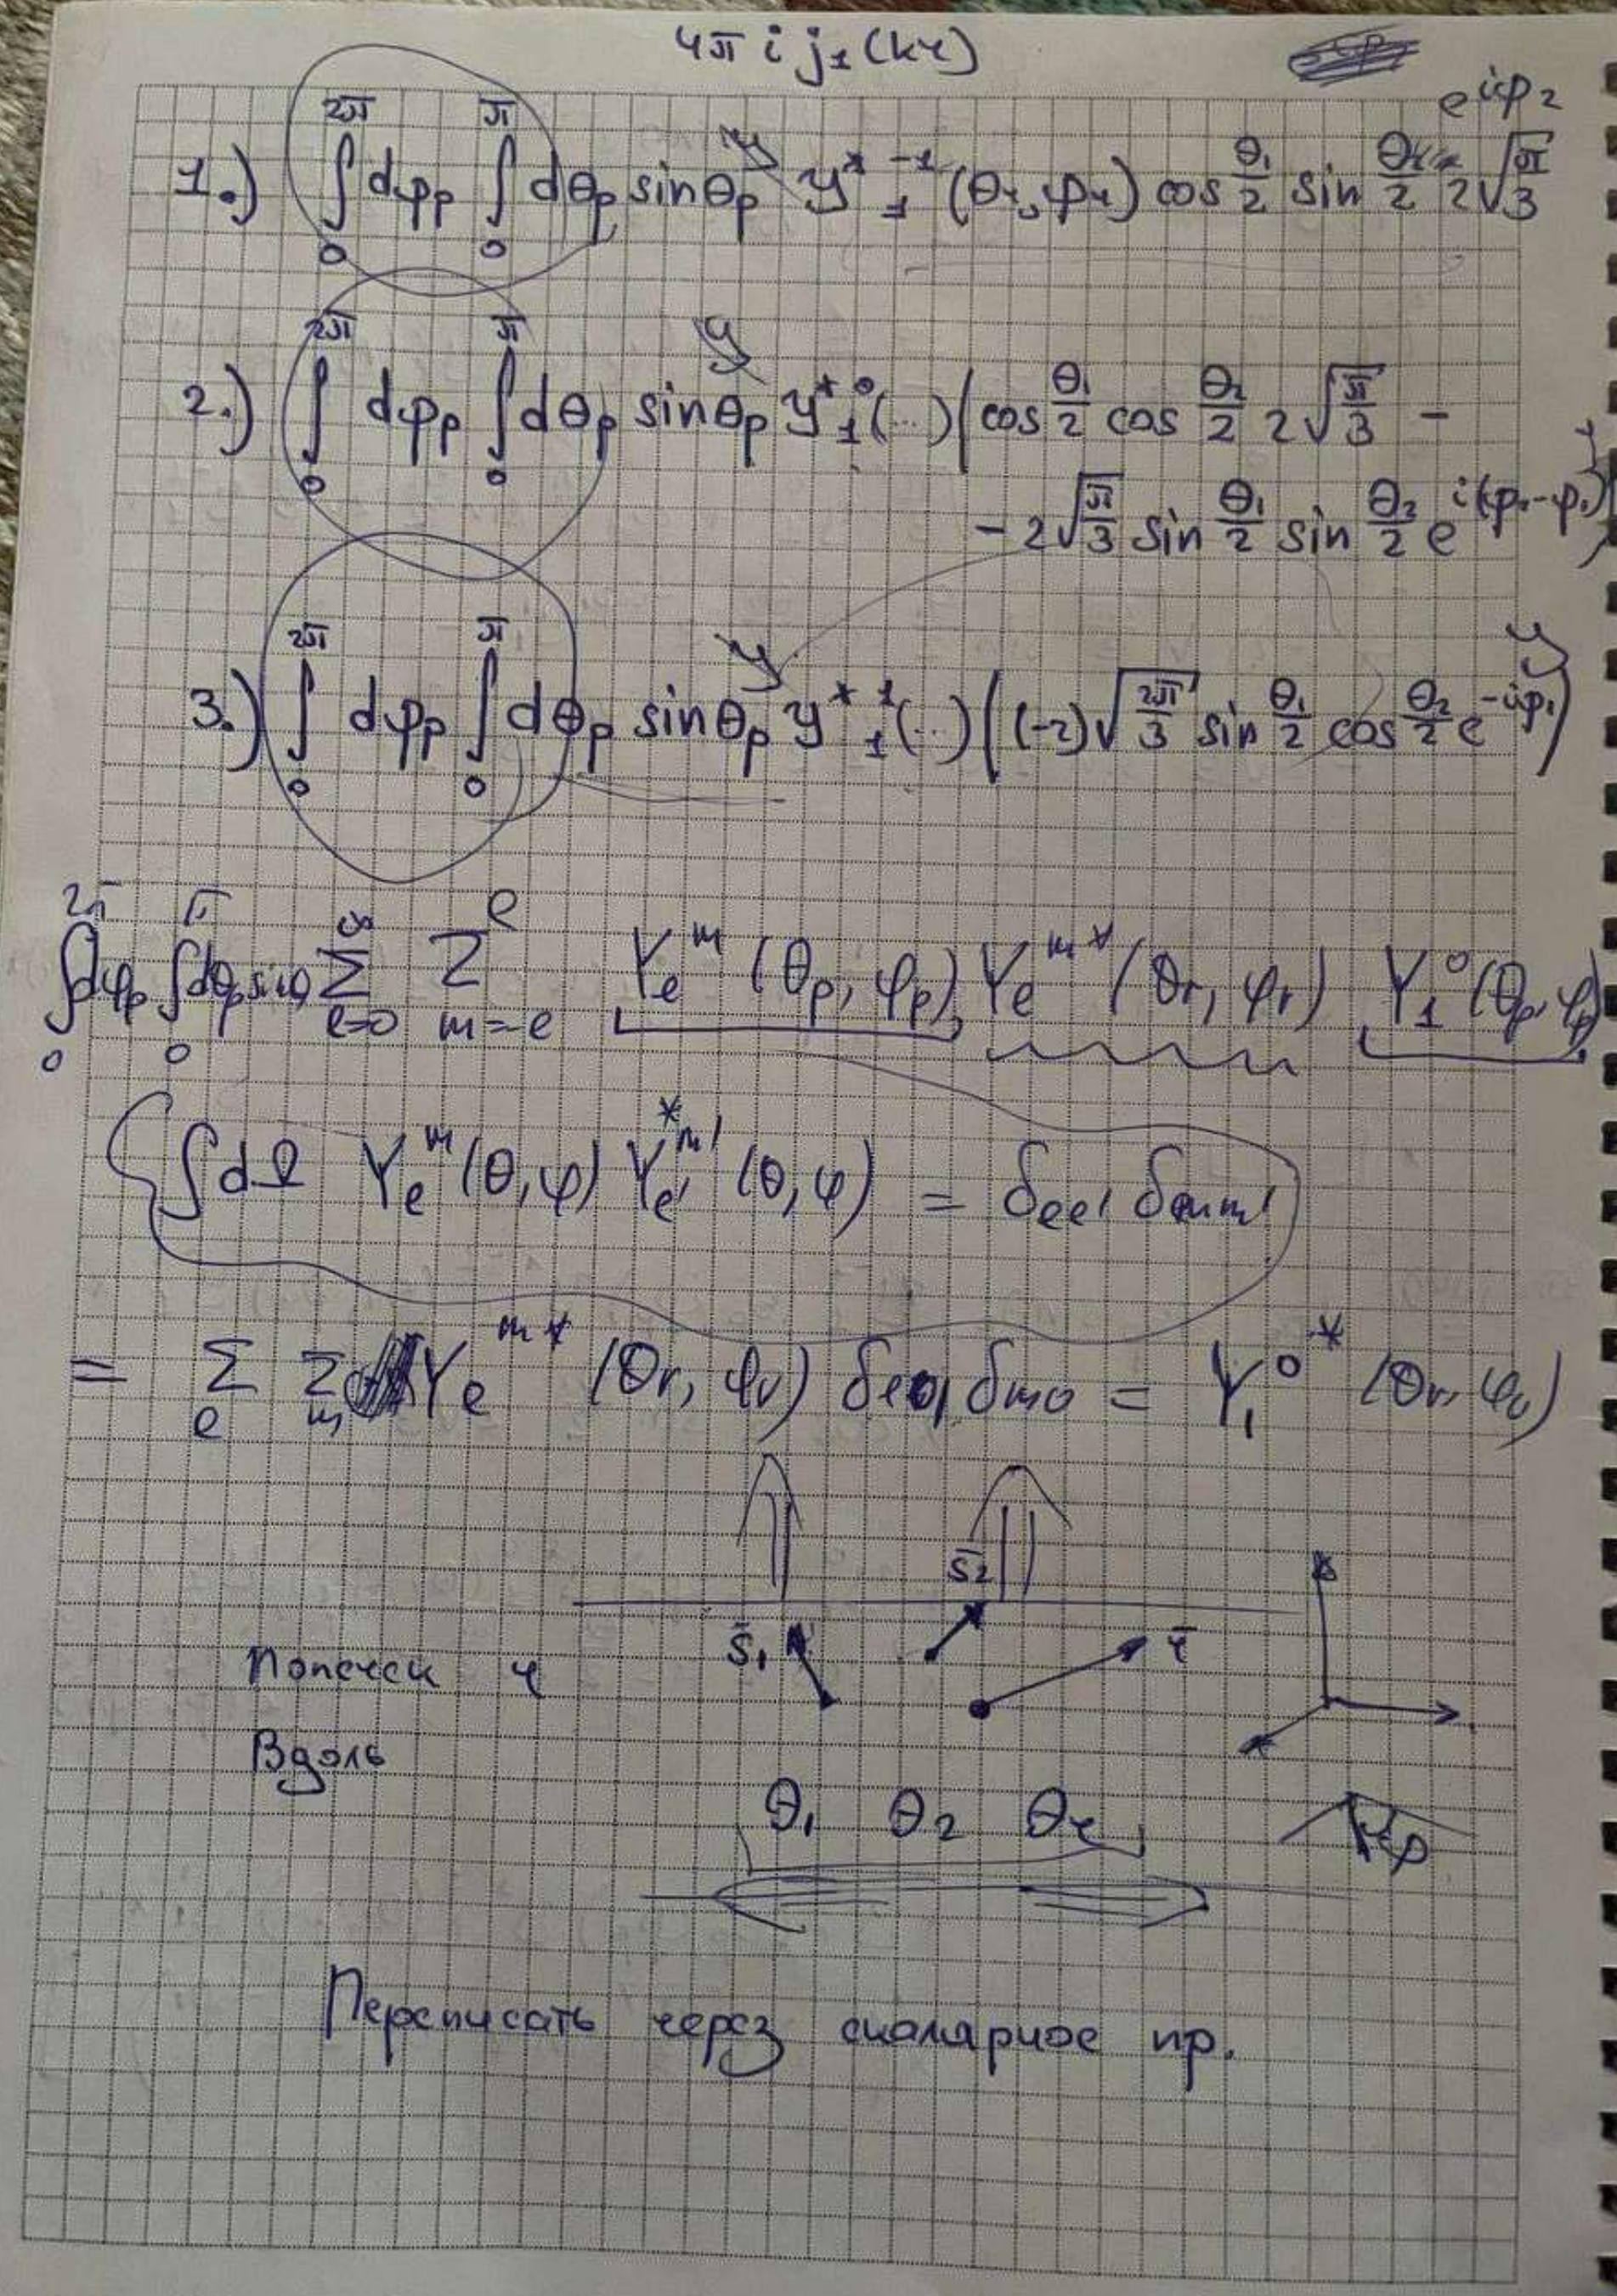
\includegraphics[max width=\textwidth, center]{2025_07_22_dcbd22cba3b771cfb453g-13}\\
\(\bar{a} \cdot \bar{b}=\cos \theta_{a b}=\cos \theta_{a} \cos \theta_{b}-\sin \theta_{a} \theta_{b} \cos \left(p_{a}-\varphi_{b}\right)\)\\
\(\Psi(s, s, y) \sim N \int_{1}(u 4)\left[2 \sqrt{3} \cos \frac{\theta_{1}}{2} \cos \frac{\theta_{2}}{2}-2 \sqrt{\frac{\pi}{3}} \sin \frac{\theta_{1}}{2} \sin \frac{\theta_{1}}{2} e d(\varphi-p)\right)\).\\
\(\psi\left(s_{1} s_{2}, r\right) \sim N j_{1}\left(k_{4}\right)\left[2 \sqrt{\frac{\pi}{3}} \cos \frac{\partial_{1}}{2} \sin \frac{\theta_{2}}{2} e^{i \varphi_{2}} y_{1}^{*-1}\left(\theta_{1}, \varphi_{1}\right)+\right.\)\\
\(y_{1\left(\theta_{1}\right)\left(\cos \frac{\theta_{1}}{2} \cos \frac{\theta_{2}}{2} 2 \sqrt{\frac{\pi}{3}}-2 \sqrt{\frac{\pi}{3}} \sin \frac{\theta_{1}}{2} \sin \frac{\theta_{2}}{2} e^{i\left(\varphi_{2}-\varphi_{1}\right)}\right)+}\)\\
\(\left.+\left((-2) \sqrt{\frac{2 \pi}{3}} \sin \frac{\theta_{1}}{2} \cos \frac{\theta_{2}}{2} e^{-i \varphi_{1}}\right) y_{1}^{* 1}\left(\theta_{2}, \varphi_{4}\right)\right]\)\\
1.\\
2. \(\cos \frac{\theta_{1}}{2} \cos \frac{\theta_{2}}{2} 2 \sqrt{\frac{\theta^{1}}{3}}-2 \sqrt{\frac{r_{1}}{3}} \sin \frac{\theta_{1}}{2} \sin \frac{\theta_{2}}{2} x\)

\[
x\left(\cos \left(\varphi_{2}-\varphi_{1}\right)+i \sin \left(\varphi_{2}-\varphi_{1}\right)\right)=
\]

\(=\cos \frac{\theta_{1}}{2} \cos \frac{\theta_{2}}{2} 2 \sqrt{\frac{\pi}{3}}-2 \sqrt{\frac{\pi}{3}} \sin \frac{\theta_{1}}{2} \sin \frac{\theta_{2}}{2} \cos \left(\phi_{2}-\phi_{1}\right)-\)

\[
-2 \sqrt{\frac{\pi}{3}} \sin \frac{\theta_{1}}{2} \sin \frac{\theta_{2}}{2} i \sin \left(\varphi_{2}-\varphi_{1}\right)
\]

\(=\bar{s}_{1} \cdot \bar{s}_{2} \cdot 2 \sqrt{\frac{\sigma^{2}}{3}}-2 \sqrt{\frac{\sigma^{3}}{3}} i \sin \frac{\theta_{1}}{2} \sin \frac{\theta_{2}}{2} \sin \left(\phi_{2}-\phi_{1}\right)\)


\end{document}